\iffalse
Title: Monoids. What, how and why?
Titulo: Monoides. Que, Como e Por Que?

Abstract:
We will learn about Monoids, a concept invented (discovered?) by mathematicians
that we can leverage to great value in our code and designs.

The talk is structured in two sessions, in this first one (5/29) we'll learn what
Monoids are, go through many examples, and write code that creates and uses Monoids. In
the second session (June maybe?) we will see how we can use Monoids to guide software design.

Despite the weird name, Monoids are easy to understand, and once you do, you'll
start finding them everywhere. More importantly, after a little practice
you'll gain intuition and you'll be able to integrate Monoids in your code and
designs, obtaining more abstract and reusable results.

Requirements:
This is an intermediate level talk. No knowledge of math or functional
programming is required. I'll assume you can understand simple Scala code.
In particular, if you don't know what implicit parameters are, spend 10 minutes
learning about them. You don't need to understand the details of implicit search
mechanisms or anything like that.


Resumo:
Vamos aprender sobre Monoids, um conceito inventado (ou descoberto?) pelos
matematicos, que nos podemos aproveitar com grandes resultados no nosso codigo e desenhos.

A palestra esta estruturada em duas sessoes, na primeira (29/05) vamos aprender o
que sao os Monoids, ver muitos exemplos e escrever codigo que cria e usa
Monoids. Na segunda sessao (data a confirmar) vamos ver como podemos usar os
Monoids para guiar o desenho de software.

Apesar de seu nome estranho, os Monoids sao faceis de entender, e uma vez que os
entenda, voce vai acha-los em todo lugar. Ainda mais importante, com um
pouco de pratica, voce vai aprimorar sua intuicao e sera capaz de integrar Monoids no seu
codigo e desenhos, consiguindo resultados mais abstratos e reusaveis.

Requerimentos:
Essa e uma palestra de nivel intermediario. Nao precisa conhecimentos de
matematica ou programacao funcional. Todos os exemplos serao em Scala, voce devera
conhecer a linguagem para entende-los. Particularmente, se voce nao sabe o que sao os parametros
implicitos, gaste 10 minutos aprendedo-os. Nao precisa saber os detalhes dos
mecanismos de busca de implicitos.
\fi

\documentclass{beamer}

\mode<presentation>
{
  \usetheme{Madrid}      % or try Darmstadt, Madrid, Warsaw, ...
  \usecolortheme{default} % or try albatross, beaver, crane, ...
  \usefonttheme{default}  % or try serif, structurebold, ...
  \useoutertheme{default}
  \setbeamertemplate{navigation symbols}{}
  \setbeamertemplate{caption}[numbered]
  \logo{\includegraphics[height=0.8cm]{assoc2.png}}
}


\usepackage[english]{babel}
\usepackage[utf8]{inputenc}
\usepackage{listings}
\usepackage{color}
\usepackage{ulem} % for \sout
\usepackage{tikz}
\usepackage{amsmath}

\title[Monoids]{MONOIDS}
\subtitle{\textit{What}, \textit{How} and \textit{Why}}
\author{Sebastian Galkin}
\institute[@paraseba]{\texttt{@paraseba} \\ \texttt{paraseba@gmail.com}}
\date[Scaladores]{Scaladores - May 2018}

\definecolor{keyword}{rgb}{0,0.38,0}
\definecolor{comments}{rgb}{0.4,0.1,0.1}

\begin{document}
\lstset{
  language=Scala,
  basicstyle={\small\ttfamily},
  keywordstyle=\color{keyword},
  commentstyle={\color{comments}\itshape},
  columns=fullflexible
}

\begin{frame}
  \titlepage
\end{frame}

% Uncomment these lines for an automatically generated outline.
\begin{frame}
  \frametitle{Outline}
 \tableofcontents
\end{frame}


\begin{frame}
  \frametitle{About me}

  {\LARGE Sebastian Galkin}

  \begin{itemize}
  \item \alert{Functional Programming} for a while.
  \item Mostly big data and enterprise.
  \item People are still scared of FP.
  \item You or your team want to learn FP?
  \color{blue}\texttt{paraseba@gmail.com}
  \end{itemize}


\end{frame}

\section{Monoids in Math \& Programming}
\subsection{Abstraction}

\begin{frame}
  \frametitle{What is Abstraction?}
  \begin{quote}
\alert{Abstraction} is the process of extracting the underlying \alert{essence} of a concept,
removing any \alert{dependence} on real world objects, and \alert{generalizing} it so that it
has \alert{wider applications.}\\[2ex] \rightline
  {{\rm --- Wikipedia, \href{https://en.wikipedia.org/wiki/Abstraction_(mathematics)}{\underline{Abstraction (mathematics)}}}}
  \end{quote}
\end{frame}

\begin{frame}
  \frametitle{You call this abstraction?}
  \begin{quote}
    I wouldn't really think of abstraction as a mathematical concept. \\[1ex] \rightline
  {{\rm --- Fishtoaster,
      \href{https://softwareengineering.stackexchange.com/questions/16070/what-is-abstraction}{\underline{SE Stack Exchange}}}}
  \end{quote}

  \begin{quote}
    A programming abstraction is a simplified model of a problem. \\[1ex] \rightline
  {{\rm --- C. Ross,
      \href{https://softwareengineering.stackexchange.com/questions/16070/what-is-abstraction}{\underline{SE Stack Exchange}}}}
  \end{quote}

  \pause

  \begin{block}{These are not abstraction}
  \begin{itemize}
    \item Inheritance.
    \item Factoring out common code to a function.
    \item Passing to functions only what they need.
  \end{itemize}
  \end{block}

  Really, how abstract is your code?

  \begin{center}
    \LARGE
    \bfseries
  We suck at abstraction!
  \end{center}

\end{frame}

\begin{frame}
  \frametitle{Standing On the Shoulders of Giants}
  Mathematicians are the \alert{masters of abstraction.}
  \begin{itemize}
  \item Maximize generality.
  \item Analogies and analogies between analogies.
  \item Reusing whole theories.
  \item Finding ``the right'' level of abstraction.
  \end{itemize}

  \pause

  \begin{center}
    \Large
    \bfseries
  This is what they have been doing for centuries.
  \end{center}

  \begin{block}{}
  copy steal copy steal copy steal
  copy steal copy steal copy steal
  copy steal copy steal copy steal
  copy steal copy steal copy steal
  copy steal copy steal copy steal
  copy steal copy steal copy steal
  copy steal copy steal copy steal
  \end{block}

\end{frame}


\subsection{What is a Monoid}

\begin{frame}
  \frametitle{What Is a Monoid?}
  \begin{block}{Monoid}
    A \alert{set} together with an \alert{associative} \alert{operation}
    and an \alert{identity} element.
  \end{block}

  \pause

  \begin{block}{Components - A Triplet \((A, \bullet, u)\)}
  \begin{itemize}
    \item A [carrier] set (\(A\))
    \item A binary operation (\(\bullet\))
    \item An element of the set \(u\)
  \end{itemize}
  We sometimes say ``\(A\) \emph{has} a Monoid''.
  \end{block}

  \pause
  \begin{block}{Laws (\(a,b,c \in A\))}

  \begin{description}[Commutativity:]
    \item[Closure:] \(a \bullet b\) is an element of \(A\)
    \item[Associativity:] \((a \bullet b) \bullet c = a \bullet (b \bullet c)\)
    \item[Identity:] \(u \bullet a = a \bullet u \ = a\)
    \item[\sout{Commutativity:}] \(a \bullet b \neq b \bullet a\)
  \end{description}
  \end{block}
\end{frame}


\subsection{Examples in math}
\begin{frame}\frametitle{A Monoid in ``Real Life''}
  Color addition

  \begin{columns}[c]
    \column{0.7\textwidth}
      \begin{itemize}
        \item \(A\): the set of all colors
        \item \(a \bullet b\): color formed adding light of color \(b\) on top
          of light of color \(a\)
        \item \(u\): transparent color
      \end{itemize}

    \column{0.3\textwidth}

    \begin{figure}
        \centering
        \def\svgwidth{\columnwidth}
        \input{additive-color.pdf_tex}
    \end{figure}
  \end{columns}

  \begin{block}{Quiz}
  What does associativity mean?
  \end{block}

  \begin{block}{Quiz}
  Is it a commutative monoid?
  \end{block}

\end{frame}

\begin{frame}\frametitle{Examples of Monoids in Math}
  \begin{itemize}
    \item Integers under addition with zero identity.
      \[
      (a + b) + c = a + (b + c) \qquad a + 0 = 0 + a = a
      \]
    \item Reals under multiplication with 1 identity.
      \[
        (a b) c = a (b c) \qquad a \times 1 = 1 \times a = a\]
    \item Subsets of a set under union with empty identity.
      \[
        \mathcal
        (\mathcal{A} \cup \mathcal{B})\cup  \mathcal{C} = \mathcal{A}\cup  (\mathcal{B}\cup  \mathcal{C}) \qquad
        \mathcal{A} \cup \emptyset = \emptyset \cup \mathcal{A} = \mathcal{A}
      \]
    \item Spatial transformations
  \end{itemize}
  \begin{block}{Quiz}
    Positive integers under division?
  \end{block}
\end{frame}

\subsection{Examples in code}

\begin{frame}\frametitle{Basic Monoids in Programming}
  \begin{itemize}
    \item<1-> \texttt{Integer} under \texttt{(+)} with \texttt{0}.
    \item<1-> \texttt{Integer} under \texttt{(*)} with \texttt{1}.
    \item\only<1>{\texttt{Double} under \texttt{(+)} with \texttt{0}?}
         \only<2->{\alert{\sout{\texttt{Double} under \texttt{(+)} with \texttt{0}}}
           \hspace{2em}
      \( (0.1+0.2)+0.3 \neq 0.1+(0.2+0.3)\).}
    \item<3-> \texttt{Boolean} under \texttt{||} with \texttt{False}.
    \item<3-> \texttt{Boolean} under \texttt{\&\&} with \texttt{True}.
    \item<3-> \texttt{Set[A]} under \texttt{union}.
  \end{itemize}

  \begin{block}{Quiz}<3->
    \begin{itemize}
    \item Is \texttt{Set[A]/union} commutative?
    \item How about \texttt{Map[K,V]/++}?
    \end{itemize}
  \end{block}
  \end{frame}

\begin{frame}[fragile]\frametitle{Modeling Monoids in Scala}
  If the type \texttt{A} \emph{has} a monoid we need:
  \begin{itemize}
    \item a way to create an \texttt{A} from nothing,
    \item a way to combine two \texttt{A}s.
  \end{itemize}

  \begin{block}{}
  \begin{lstlisting}
trait Monoid[A] {

  // The associative operation
  def append(a: A, b: => A): A

  // The identity
  def zero: A
}
  \end{lstlisting}
  \end{block}

  We can have more than one Monoid for the same \texttt{A}
\end{frame}

\begin{frame}[fragile]\frametitle{Two Monoids for Ints}
  \begin{block}{}
  \begin{lstlisting}
val sumMon = new Monoid[Int] {
  def zero: Int = 0

  def append(a: Int, b: => Int): Int =
    a + b
}

val mulMon = new Monoid[Int] {
  def zero: Int = 1

  def append(a: Int, b: => Int): Int =
    a * b
}
  \end{lstlisting}
  \end{block}
  These Monoid \alert{instances} are first class citizens
\end{frame}

\begin{frame}[fragile]\frametitle{The List Monoid}
  \begin{block}{}

  \begin{lstlisting}
implicit val freeMon[A] = new Monoid[List[A]] {

  def zero: List[A] = List()

  def append(as: List[A], bs: => List[A]): List[A] =
    a ++ b

}
  \end{lstlisting}
  \end{block}

  \begin{block}{Quiz}
Is it a commutative monoid?
  \end{block}
\end{frame}

\begin{frame}[fragile]\frametitle{Monoid for Tuples}
  How can we combine two tuples \texttt{(A,B)}?
  \pause

  If \texttt{A} and \texttt{B} have monoids themselves, we can \alert{combine componentwise}.

  \begin{block}{}
  \begin{lstlisting}
def pairMon[A: Monoid, B: Monoid]: Monoid[(A,B)] =
  //(implicit am: Monoid[A], implicit bm: Monoid[B])

  new Monoid[(A, B)] {
    val am = implicitly[Monoid[A]]
    val bm = implicitly[Monoid[B]]

    def zero: (A,B) = (am.zero, bm.zero)

    def append(a: (A, B), b: => (A, B)): (A,B) =
      (am.append(a.fst, b.fst), bm.append(a.fst, b.fst))
  }
  \end{lstlisting}
  \end{block}

  \texttt{am} and \texttt{bm} are sometimes called \emph{evidence} or
  \emph{witnesses} of the monoids for \texttt{A} and \texttt{B}.
\end{frame}


\begin{frame}[fragile]\frametitle{Is There a Monoid for Functions?}
  It seems hard for arbitrary functions \texttt{A => B}.
  \pause
  But how about \alert{\texttt{A => A}}?

  \pause
  \begin{block}{Functions that take and return the same type}

  \begin{lstlisting}
def endoMon[A]: Monoid[A => A] = Monoid[A => A] {

  def zero: A => A = identity

  def append(f: A => A, g: => (A => A)): A => A =
    g andThen f  // function composition is associative

}
  \end{lstlisting}
  \end{block}
  \begin{block}{Quiz}
    \begin{itemize}
      \item Is it a commutative Monoid?
      \item Can we do \texttt{(f andThen g)} instead?
    \end{itemize}
  \end{block}
\end{frame}


\begin{frame}[fragile]
  \frametitle{A Different Monoid for Functions}
  How about \texttt{A => B} where \alert{\texttt{B} has a Monoid?}

  \begin{block}{Functions that return a monoidal type}
  \begin{lstlisting}
def monFunMon[A, B: Monoid]: Monoid[A => B] =
    new Monoid[A => B] {

      val bMon = implicitly[Monoid[B]]

      def zero: A => B = _ => bMon.zero

      def append(f: A => B, g: => (A => B)): A => B =
        a => bMon.append(f(a), g(a))
  }
  \end{lstlisting}
  \end{block}
  Convince yourself \texttt{append} is associative.
\end{frame}

\begin{frame}[fragile]
  \frametitle{Option Monoids}
  \begin{onlyenv}<1>
  \begin{block}{Quiz}
    Would it make sense to try to write an instance of
    \texttt{Monoid[Option]}
  \end{block}
  \end{onlyenv}

  \begin{onlyenv}<2>
    There are several ways to combine \texttt{Options[A]}

  \begin{block}{Taking the first \texttt{Some}}
  \begin{lstlisting}
def firstMon[A]: Monoid[Option[A]] = new Monoid[Option[A]] {

  def zero: Option[A] = None

  def append(a: Option[A], b: => Option[A]): Option[A] =
    a orElse b
}
  \end{lstlisting}
  \end{block}

  Similarly taking the last \texttt{Some}
  \end{onlyenv}

\end{frame}


\begin{frame}[fragile]
  \frametitle{Option Wrapping a Monoidal Type}
  \begin{block}{Using the wrapped monoid}
  \begin{lstlisting}
def weird[M: Monoid]: Monoid[Option[M]] = new Monoid[Option[M]] {
  def zero: Option[M] = None  // weird!
  def append(a: Option[M], b: => Option[M]): Option[M] =
    (a,b) match {
      case (a, None) => a
      case (None, b) => b
      case (Some(a),Some(b)) =>
        Some(implicitly[Monoid[M]].append(a, b))
      }
}
  \end{lstlisting}
  \end{block}

  \begin{block}{Quiz}
    \begin{itemize}
      \item Why is \texttt{zero} weird?
      \item Can we do \texttt{zero = Some(m.zero)} instead?
    \end{itemize}
  \end{block}
\end{frame}

\begin{frame} \frametitle{Recap}
  We have seen:
  \begin{itemize}
    \item Monoid definition (binary assoc operation with identity).
    \item Monoid \texttt{trait} (one type parameter,
      two methods: \texttt{zero, append})
    \item Monoids for:
      \begin{itemize}
      \item Numbers, lists, tuples (if members have monoids)
      \item \texttt{A => A} and \texttt{A => M} where \texttt{M} has a monoid
      \item \texttt{Options} (first, last and Monoid wrapper)
      \item There are many, many more.
      \end{itemize}
  \end{itemize}

  \begin{block}{}
    \centering
    But we haven't seen \alert{why} or \alert{how} to use monoids.
  \end{block}
\end{frame}

\subsection{Usage}
\begin{frame}[fragile]
  \frametitle{Simple usage examples}

  \begin{block}{A useful function: \texttt{mconcat}}
  \begin{lstlisting}
def mconcat[A: Monoid](as: List[A]): A = {
  val m = implicitly[Monoid[A]]

  // fold? foldLeft? foldRight? What laws are we using?
  as.fold(m.zero)(m.append(_, _))
}

def sum(xs: List[Int]): Int = mconcat(xs)(sumMon)

def first[A](os: List[Option[A]]): Option[A] =
  mconcat(os)(firstMon)
  \end{lstlisting}
  \end{block}

  \begin{block}{Super useful. MapReduce}
  \begin{lstlisting}
def foldMap[A, M: Monoid](List[A])(f: A => M): M
  \end{lstlisting}
  \end{block}
  See \texttt{Foldable}.
\end{frame}

\begin{frame}[fragile]{Composing Monoids}

  \begin{block}{Define a comparison}
  \begin{onlyenv}<1>
  \begin{lstlisting}[escapechar=\|]
sealed trait Ord[A] {
  def compare(a: A,  b:A): |\fbox{\texttt{???}}|
}
\end{lstlisting}
\end{onlyenv}

\begin{onlyenv}<2>
\begin{lstlisting}[escapechar=\|]
sealed trait Ord[A] {
  def compare(a: A,  b:A): |\fbox{\texttt{Ordering}}|
}

sealed trait Ordering

object Ordering {
  case object LT extends Ordering
  case object GT extends Ordering
  case object EQ extends Ordering
}

  \end{lstlisting}
  \end{onlyenv}
  \end{block}

  \only<1>{What should we use for \fbox{???} here?}
\end{frame}

\begin{frame}[fragile]
  \frametitle{Composing Monoids}
  It turns out \texttt{Ordering} has a monoid:

  \begin{block}{An \texttt{Ordering} monoid}
  \begin{lstlisting}
val ordMon = new Monoid[Ordering] {
  def zero: Ordering = Ordering.EQ

  def append(a: Ordering, b: => Ordering): Ordering =
    a match {
      case Ordering.EQ => b
      case o => o
  }
}
  \end{lstlisting}
  \end{block}
\end{frame}

\begin{frame}[fragile]
  \frametitle{Composing Monoids}
  \begin{block}{}
  \begin{lstlisting}
def sortBy(as: Array[A])(by: A => A => Ordering): Array[A] = ...
def comparing[A, B](f: B => A)(b1: B, b2: B)(implicit o: Ord[A]): Ordering

case class Person(addr: Address, name: String, dob: Date)
case class Address(zip: Int, street: String)

val people: Array[Person] = ...

val sorted = sortBy(people)(mconcat(List(
  comparing(_.address.zip),
  comparing(_.name),
  comparing(_.dob)))

  \end{lstlisting}
  \end{block}
\end{frame}

\begin{frame}
  \frametitle{Larger Use Cases}
  \framesubtitle{Parallelization}
  \[a_1 \bullet a_2 \bullet a_3 \dotsb \bullet a_n\]

  What happens if \texttt{append} for \texttt{Monoid[E]} is CPU expensive?

\pause
% Copyright 2018 Sebastian B. Galkin

% This file is part of paraseba/scaladores-may-2018-talk.

% paraseba/scaladores-may-2018-talk is free software: you can redistribute it and/or modify
% it under the terms of the GNU General Public License as published by
% the Free Software Foundation, either version 3 of the License, or
% (at your option) any later version.

% paraseba/scaladores-may-2018-talk is distributed in the hope that it will be useful,
% but WITHOUT ANY WARRANTY; without even the implied warranty of
% MERCHANTABILITY or FITNESS FOR A PARTICULAR PURPOSE.  See the
% GNU General Public License for more details.

% You should have received a copy of the GNU General Public License
% along with Foobar.  If not, see <http://www.gnu.org/licenses/>.

\begin{center}
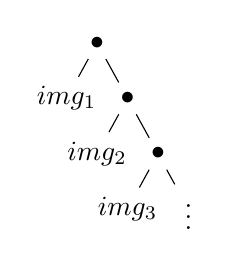
\begin{tikzpicture}[sibling distance=2.2em, level distance=2em]
  \node {\(\bullet\)}
    child { node {\(img_1\)} }
    child { node {\(\bullet\)}
      child { node {\(img_2\)}}
      child { node {\(\bullet\)}
        child { node {\(img_3\)}}
        child { node {\(\vdots\)}
    }}};
\end{tikzpicture}
\qquad
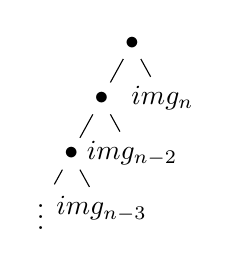
\begin{tikzpicture}[sibling distance=2.2em, level distance=2em]
  \node {\(\bullet\)}
    child { node {\(\bullet\)}
      child { node {\(\bullet\)}
        child {node {\(\vdots\)}}
        child {node {\(img_{n-3}\)}}}
      child { node {\(img_{n-2}\)}}
        }
    child { node {\(img_n\)} };
\end{tikzpicture}
\qquad
\begin{tikzpicture}[level distance=2em, level 3/.style={sibling distance=3em}, level 2/.style={sibling distance=2.5em}, level 1/.style={sibling distance=6em}]
  \usebeamercolor{example text}
  \node {\(\bullet\)}
  child { node[color=fg] {\(\bullet\)}
    child { node[color=fg] {\(\bullet\)}
      child {node[color=fg] {\texttt{zero}}}
      child {node[color=fg] {\(img_1\)}}}
    child { node[color=fg] {\(img_2\)}}
  }
  child { node[color=red] {\(\bullet\)}
    child { node[color=red] {\(img_3\)} }
    child { node[color=red] {\(\bullet\)}
      child { node[color=red] {\(img_4\)}}
      child { node[color=red] {\(\vdots\)}
      }}};
\end{tikzpicture}
\end{center}

\begin{block}{Quiz}
  \pause
  Can we swap the two red root branches in the last tree?
\end{block}

\end{frame}

\begin{frame}
  \frametitle{Larger Use Cases}
  \framesubtitle{Incremental updates}
  The Problem:

  \begin{itemize}
    \item System measures a magnitude (e.g. latency)
    \item Compute and store daily means, variances, etc.
    \item Events arrive at high rate (millions per hour)
  \end{itemize}


\end{frame}

\begin{frame}
  \frametitle{Larger Use Cases}
  \framesubtitle{Incremental updates}
  \begin{columns}[c]
    \column{0.6\textwidth}
      \begin{block}{Naive approach}
        \begin{itemize}
        \item On event load all previous measurements,
        \item recompute meand/variance,
        \item store.
        \end{itemize}
      \end{block}

    \column{0.3\textwidth}
  Too much \alert{memory}, to much compute \alert{time}, not able to \alert{catch up}
  to the stream.
  \end{columns}

  \pause

  \begin{columns}[c]
    \column{0.6\textwidth}
      \begin{block}{Unsound approach}
        \begin{itemize}
        \item Store previous mean/variance,
        \item on event, average previous and current,
        \item store.
        \end{itemize}
      \end{block}

    \column{0.3\textwidth}
    Fast, low memory. But, if we got \(2,1\) and then \(0\):

    \alert{\(\frac{(2 + 1) / 2 + 0}{3} \neq 1\).}
  \end{columns}
\end{frame}

\begin{frame}
  \frametitle{Larger Use Cases}
  \framesubtitle{Incremental updates}
  A better approach (showed for mean but easy to generalize):

  \begin{itemize}
  \item Store mean and number of measurements
  \item accumulate several (or 1) new events,
  \item combine the old and new means using the right \alert{monoid},
  \item store.
  \end{itemize}

\end{frame}

\begin{frame}
  \frametitle{Larger Use Cases}
  \framesubtitle{Incremental updates}
  What to store?
  \[
  \begin{split}
    \mu = \sum_{i=0}^{n-1} x_i \qquad  \nu = \sum_{i=0}^{m-1} x_{i+n} \\
    \frac{1}{n+m} \sum_{i=0}^{n+m-1} x_i = \frac{n\mu + m\nu} {n+m}
  \end{split}
  \]

  \pause

  \begin{itemize}
  \item Store mean and number of measurements
  \item accumulate several (or 1) new events,
  \item combine the old and new means using the right \alert{monoid},
  \item store.
  \end{itemize}
\end{frame}

\begin{frame}[fragile]
  \frametitle{Larger Use Cases}
  \framesubtitle{Incremental updates}
  \begin{block}{The mean monoid}
  \begin{lstlisting}
case class Mean(mu: Double, n: Int)

implicit val meanMonoid = new Monoid[Mean] {
  def zero: Mean = Mean(0,0)

  def append(a: Mean, b: => Mean): Mean = (a, b) match {
     case (Mean(mua, na), Mean(mub, nb)) =>
       Mean((mua * na + mub * nb) / (na + nb), na + nb)
  }
}
  \end{lstlisting}
  \end{block}
  Now we can accumulate measurements for some time, and then easily
  combine the previous stored averages with new ones.
\end{frame}

\begin{frame}
  \frametitle{Larger Use Cases}
  \framesubtitle{Incremental updates}
  Few more details:
  \begin{itemize}
    \item How about \texttt{Double} under sum not being a monoid?
  \item We saw mean, but same is extensible to variance.
  \item In fact, it's extensible to any higher moment.
  \item In fact, you can extend it to do approximate histograms and other fun stuff.
  \end{itemize}

\end{frame}

\subsection{References}

\section{Monoids in Design \color[rgb]{0.5,0.1,0.9}[next session]}



% \begin{frame}{Functional Programming in Scala}
%   reading the book as a group?
% \end{frame}

% \begin{frame}{Figures as Monoids Paper}
% \end{frame}

% \begin{frame}{Why functional programming matters}
% \end{frame}

% \begin{frame}{Scalaz}
% \end{frame}



\begin{frame}{ToDo / Fixme}
  \begin{itemize}
    \item what happens with broken rules
    \item Monoid seems too simple but it's powerful
    \item mconcat can be parallelized, incrementally, cached
    \item dual monoid
    \item summaries
      \item substracition not a monoid
      \item where to find code/presentation
        \item mathematical building, is elegant, if you don't care about
          elegance in software what do you care about? elegance is simple (not easy)
    \item level of the talk, audience
    \item accent
    \item quizes to keep awake
      \item scalaz to try things
        \item grammarly
          \item The Red Book
            \item syntax sugar for implicits
              \item lazyness, is the by name argument important?
                \item integer overflow is a monoid?
                  \item endo monoid composition order
                  \item either monoid?
                    \item monoid for config
  \end{itemize}
\end{frame}

\end{document}